
%===============================================================================
\section{UV emission from hot evolved stars}\label{sec:colors}
%===============================================================================

As discussed in \S\ref{sec:stars:continuum}, there are broad classes of star formation histories that produce reasonable SDSS ETG colors. Thus, the emission line ratios and equivalent widths presented in \S\ref{sec:stars} are relatively model independent, as the optical properties of ETGs are fairly well understood. The UV is much more uncertain, however, as galaxies with similar optical colors can have very different UV colors. In this section, we ask if the models from \S\ref{sec:stars} are also able to correctly predict the properties of other UV populations, including post-AGB stars, hot horizontal branch stars, and blue straggler stars. We note that the evolutionary pathways and lifetimes of these populations are not well-understood and models of their SEDs are uncertain.

In this section we explore the contribution from three main stellar types. We first consider post-AGB stars, which we have shown dominate the ionizing photon budget at old ages and are able to reproduce the emission line properties of LIER-like galaxies. We can vary the contribution from post-AGB stars to the total SED using the {\tt pagb} parameter in \FSPS. This parameter specifies the weight given to the post-AGB star phase, where {\tt pagb=0.0} turns off post-AGB stars and {\tt pagb=1.0} implies that the MIST models are implemented as-is, the default behavior in \FSPS. Models with {\tt pagb} between 0 and 1 have the flux from the post-AGB stars scaled down by {\tt pagb}.

Second, we explore the contribution from hot horizontal branch stars. These stars are not as luminous as post-AGB stars, but are longer-lived and thus more numerous. Blue horizontal branch (BHB) stars typically have temperatures between 7,000 and 20,000K \citep{Schiavon+2004}, with the hottest BHB stars often referred to as Extreme Horizontal Branch (EHB) stars. A modest population of BHB stars can alter the UV colors of a stellar population. However, since temperatures in excess of 15,000K are required to ionize hydrogen, only in the most extreme cases will BHB stars contribute significantly to the ionizing photon budget. BHB stars are not included in the default \FSPS parameters, but they can be included using the {\tt fbhb} parameter, which specifies the fraction of horizontal branch stars that are blue. \FSPS redistributes the specified fraction of HB stars such that they are uniformly spread in $\log T_{\mathrm{eff}}$ to $10^4$K \citep[e.g.,][]{Sarajedini+2007}. However, BHB temperatures have been observed in excess of $10^4$K, to include the most extreme cases we increase the BHB temperature limit to $10^{4.5}$K (${\sim}$30,000$\,$K, the limit of a B-type star) in the following tests.

Finally, we also explore the contribution from blue straggler stars. These are rejuvenated main sequence stars that appear blueward of the main sequence turn-off in globular clusters (GCs). We vary the contribution of these stars in \FSPS using the $S_{\mathrm{BS}}$, or {\tt sbss} parameter, which specifies the specific frequency of blue straggler stars relative to the number of horizontal branch stars ($S_{\mathrm{BS}} = N_{\mathrm{BS}} / N_{\mathrm{HB}}$). This number can be varied between 0 and 10, but is observed to be between 0.1 and 5 in GCs, and its value in ETGs is unknown.

In Fig.~\ref{fig:HPHB} we show an example spectrum from a 3 Gyr SSP at solar metallicity, shown in black. We indicate the ionization energies of hydrogen and helium with the black dashed lines, and show the GALEX FUV and NUV bandpasses in grey. We then systematically vary the {\tt pagb}, {\tt fbhb}, {\tt sbss} parameters from the baseline models.

We show the effect of decreasing {\tt pagb} from 1 to $10^{-1}$, $10^{-2}$, and $10^{-3}$ in orange. Scaling down the implemented post-AGB star contribution scales down the emergent EUV radiation in the spectrum. The MIST models do not include evolutionary pathways for early-AGB or AGB-Manque stars, so varying {\tt pagb} could be interpreted as varying the number of stars evolving through the traditional post-AGB phase. If a substantial fraction of post-AGB stars have untraditional evolutionary pathways, the ionizing photon budget would change significantly.

We show the effect of adding BHB stars in purple, where {\tt fbhb} is increased from 0 to 0.1, 0.5 and 1.0. Allowing hotter BHB stars does not change the ionizing photon budget but does change the UV colors dramatically. 

The addition of blue straggler stars is shown in blue, where we have increased the specific frequency {\tt sbss} from 0 to 0.1, 1, and 5. These stars are not as hot as the BHB stars, and primarily change the NUV flux. In older populations, as the main sequence turn-off evolves to cooler temperatures, the NUV contribution from BS stars should decrease.

%GCs with mostly blue HBs (asterisks) have stronger Balmer lines and thus appear younger than GCs with red HBs (open circles), even though they are all equally old Schiavon
%old hot stars that may be sufficiently bright and numerous to boost the EWs of Balmer lines, mimicking the signature of young stars in the integrated spectra of old SPs.

%-------------------------------------------------------
% Diff stellar types
%-------------------------------------------------------
\begin{figure*}
  \begin{center}
    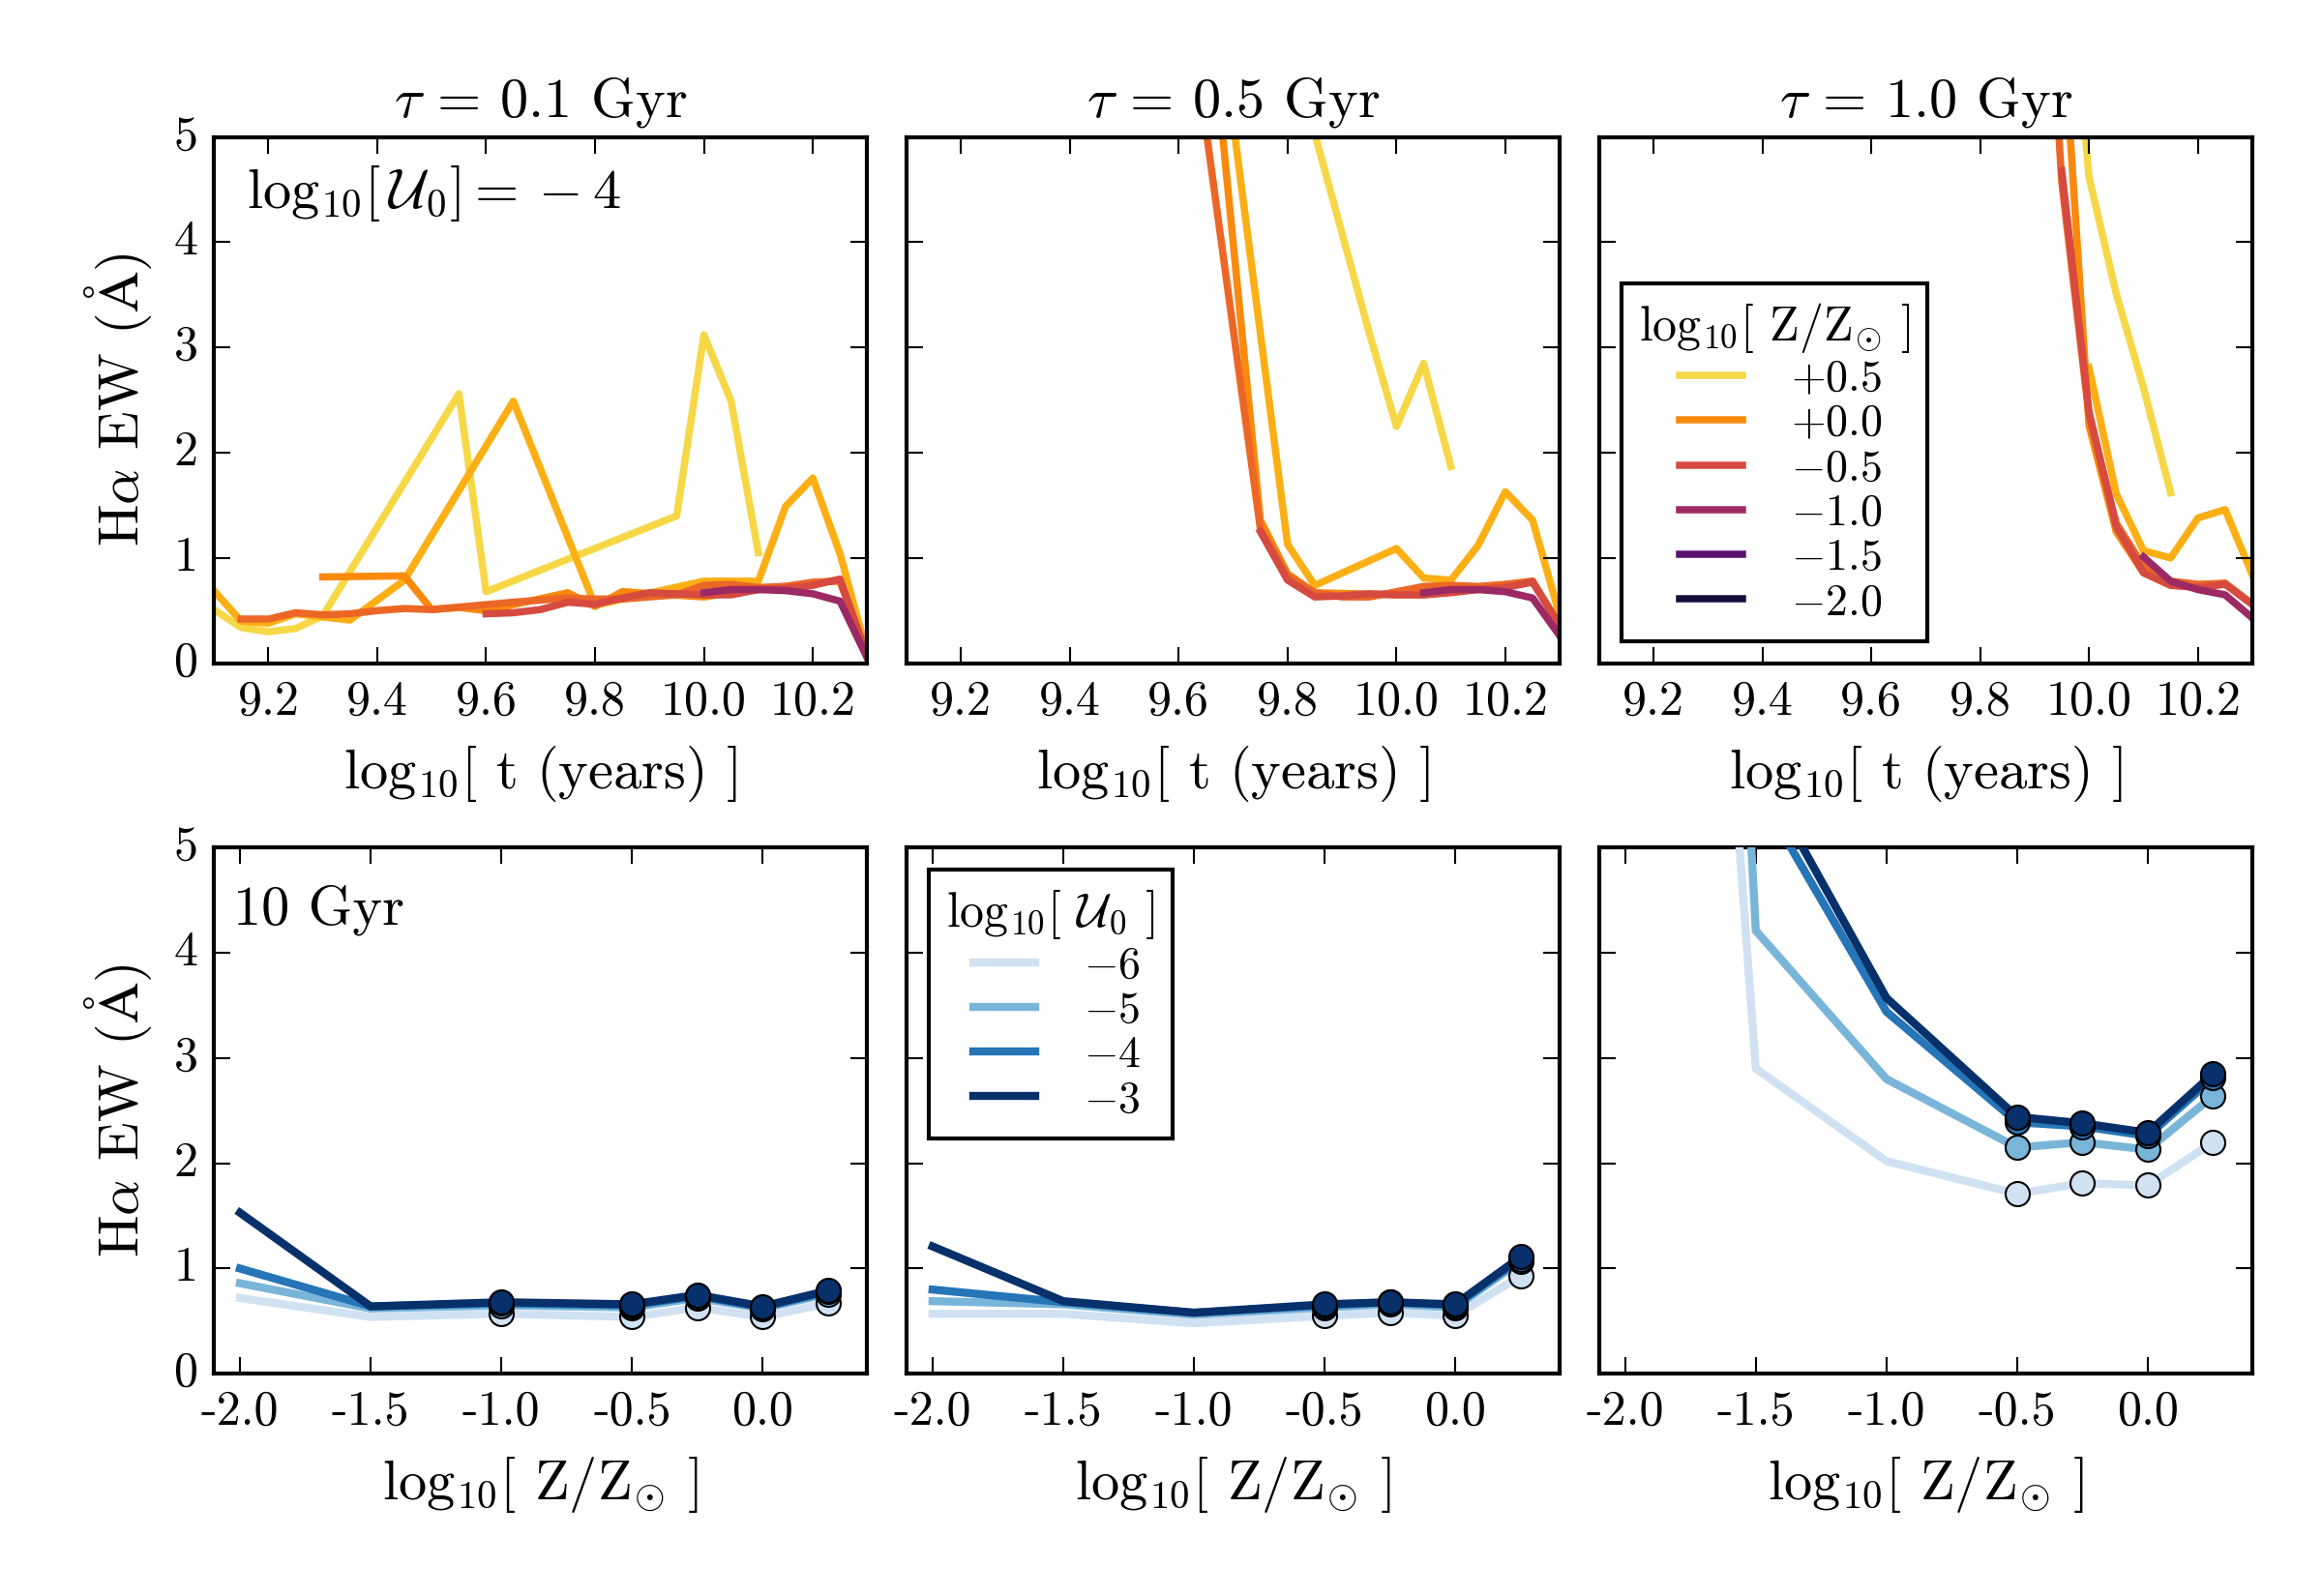
\includegraphics[width=0.7\textwidth]{figs/f13.png}
    \caption{The UV spectrum of a solar-metallicity instantaneous burst where the contribution of post-AGB stars (orange), blue HB stars (purple), and blue straggler stars (blue) are varied. The unmodified spectrum is shown in black. The post-AGB stars are responsible for the ionizing radiation responsible for producing LIER-like emission, but have little influence over the galaxy's UV colors. In contrast, the blue HB stars and blue straggler stars significantly change the UV color of the population but have little effect on the ionizing radiation output.}
    \label{fig:HPHB}
  \end{center}
\end{figure*}
%-------------------------------------------------------

\subsection{UV-upturn colors}

Fig.~\ref{fig:HPHB} suggests that the FUV and NUV properties of early type galaxies will be sensitive to the details of the post-AGB, HB, and BS populations. Models of ETG UV emission will therefore depend on exactly how these models are implemented. We first compare our baseline ETG models to GALEX observations. We then consider variations in the default \FSPS parameters that bring the models and observations into better alignment.

In Fig.~\ref{fig:UVcolors} we show the $FUV-NUV$ \emph{\vs} $NUV-r$ color evolution of our baseline ETG models as a function of SFH, age and metallicity. Just as in Fig.~\ref{fig:optCols}, each row shows a different SFH, from $\tau=0$, an instantaneous burst, to $\tau$=1\Gyr. The points are color-coded by their metallicity, and the model age is indicated by the opacity, where 13\Gyr models points are fully opaque. The left column shows models that do not include nebular emission, while the right column shows models that include the contribution from nebular line and continuum emission, assuming an ionization parameter of \logUeq{-4}.

Fig.~\ref{fig:UVcolors} is a reproduction of a figure presented in \citet{Hernandez+2014}. To appropriately compare with the \citet{Hernandez+2014} results, we adopt the same observational cut of \hb$\leq 2.1$\ang used in their work on our models. The vertical dashed line at $NUV-r$=5.4 is their galaxy red sequence limit and the horizontal line at $FUV-NUV$ = 0.9 shows the limit for selection of classical UV- upturn galaxies. Galaxies on the red sequence that fall below this line are said to have a ``UV excess'' (UVX) \citep{Smith+2014}. Galaxies below this line but on the blue side of the red sequence division are thought to have blue colors originating from residual star-formation (RSF), rather than canonical UVX emission.

The grey region in Fig.~\ref{fig:UVcolors} shows the range of UV colors observed for ETGs in the \citet{Hernandez+2014} sample. This region is most easily populated by models with high metallicity or somewhat extended SF. Though our models had very similar optical colors, they show a wide range of UV colors in Fig.~\ref{fig:UVcolors}, primarily driven any amount of recent star formation. The sustained star formation in the delayed-$\tau$ models with $\tau$=1\Gyr limited the range of ages and metallicities that could produce ETG-like colors. In Fig.~\ref{fig:UVcolors}, most of these models fall in the ``residual star formation'' section of the diagram.

We note that most of our default models (\emph{left column}) are slightly too red in $FUV-NUV$ to adequately match the \citet{Hernandez+2014} sample. This is slightly improved if we consider the models that include nebular emission (\emph{right column}), which are able to reproduce a wider range of observed ETG colors. At low metallicity however, the models with nebular emission are too blue in $NUV-r$, masquerading as galaxies with residual star formation despite their low \hb equivalent widths and old ages.

\citet{Hernandez+2014} found it difficult to generate models in the UVX portion of the UV color-color diagram without invoking binary star interactions, which can strip the outer envelope of a star, making it appear hotter. In contrast, our models are able to populate the UVX portion of Fig.~\ref{fig:UVcolors}, but only at high metallicity. It is easier to populate the UVX portion of the color-color diagram when including nebular emission, though none of our models reach the most extreme regions of the UVX region.

The default models in Fig.~\ref{fig:UVcolors} do not include BHB or BS populations, (i.e., {\tt fbhb}, {\tt sbss} $= 0$). Including these populations will add flux to the FUV and NUV bands, making $NUV-r$ and $FUV-NUV$ colors bluer. It thus seems likely that post-AGB stars are not solely responsible for the observed UV-excess in ETGs. This points to a scenario where the post-AGB stars produce the ionizing radiation necessary for LIER-like emission, while a different population of HPHB stars drive the FUV and NUV behavior.

%-------------------------------------------------------
% UV colors
%-------------------------------------------------------
\begin{figure*}
  \begin{center}
    \includegraphics[width=0.65\textwidth]{figs/f14.png}
    \caption{$FUV-NUV$ \vs NUV - r colors for our ETG models with stellar only (\emph{left column}) and stellar+nebular emission (\emph{right column}). Each row shows a different delayed$-\tau$ model: $\tau=0.0$\Gyr (instantaneous burst, \emph{top row}), $\tau=0.1$\Gyr (\emph{second row}), $\tau=0.5$\Gyr (\emph{third row}), and $\tau=1$\Gyr (\emph{bottom row}). Models with ages between 1 and 13\Gyr are plotted, color-coded by metallicity. Age is indicated by the transparency of the points, with the 13\Gyr model points fully opaque.
    The vertical dashed line at $NUV-r$=5.4 separates red-sequence galaxies, and the horizontal line at $FUV-NUV$=0.9 shows the boundary of classic UV-upturn galaxies from \citet{Smith+2014}. \citet{Hernandez+2014} further separates strong UV emitters with a FUV-r cut, shown with the grey line. To compare our models with the sample of ETGs from \citet{Hernandez+2014}, we have made the same cut in \hb equivalent width (\hb$<2.0$\ang) in our models. The inclusion of nebular line and continuum emission shifts models to both bluer $FUV-NUV$ and $NUV-r$ colors. The post-AGB stars responsible for nebular emission cannot be wholly responsible for the UV excess in some ETGs.
    }
    \label{fig:UVcolors}
  \end{center}
\end{figure*}
%-------------------------------------------------------

We show the same UV color-color diagram from Fig.~\ref{fig:UVcolors} in Fig.~\ref{fig:UVhphb}V, except now for models where we vary the various HPHB populations. We show instantaneous bursts at 8 and 13\Gyr (left and right panels, respectively), and metallicities of \logZeq{-0.5}, 0.0, and 0.25. The baseline model from Fig.~\ref{fig:UVcolors} is shown in black, for comparison. Variations due to changes in {\tt pagb} are shown in orange, changes in {\tt fbhb} are shown in purple, and changes in {\tt sbss} are shown in blue.

Variations in {\tt sbss} produce negligible changes in the ionizing spectrum at 8 and 13\Gyr, because at these late ages, the rejuvenated main sequence stars are too cool to contribute significantly to the UV flux. Variations in {\tt pagb} parameter move the models away from the observed locus of ETGs, while variations in {\tt fbhb} move the models towards the center of the observed ETG locus. For some models, even a small fraction of BHB stars (${\sim}10$\%) can successfully move the model into the UVX portion of the diagram. However, for most models, increasing {\tt fbhb} largely moves the models to bluer $NUV-r$ colors at similar $FUV-NUV$ colors, indicating that the BHB stars considered here are not hot enough to explain all ETGs with UVX emission. We note that in \FSPS, the BHB stars are evenly distributed across the horizontal branch in temperature. Models with only BHB or EHB stars could still produce the necessary FUV flux needed to move the baseline models into the UVX region.

%-------------------------------------------------------
% UV colors
%-------------------------------------------------------
\begin{figure*}
  \begin{center}
    \includegraphics[width=0.95\textwidth]{figs/f15.png}
    \caption{$FUV-NUV$ \vs NUV - r colors for our ETG models for an instantaneous burst at 8\Gyr (\emph{left}) and 13\Gyr (\emph{right}). Models are connected by lines that are color-coded by metallicity, for \logZeq{-0.5}, 0.0, and 0.25. The black marker indicates the standard stellar population, where {\tt pagb}$\,=1$ and {\tt fbhb}$\,=0$. The varying blue markers show the change in color when {\tt fbhb} is varied from the fiducial model, and the orange colored points show the change in color when {\tt pagb} is varied from the fiducial model.
    The vertical dashed line at $NUV-r$=5.4 separates red-sequence galaxies, and the horizontal line at $FUV-NUV$=0.9 shows the boundary of classic UV-upturn galaxies from \citet{Smith+2014}. \citet{Hernandez+2014} further separates strong UV emitters with a FUV-r cut, shown with the grey line.
    }
    \label{fig:UVhphb}
  \end{center}
\end{figure*}
%-------------------------------------------------------

\section{Isochrone variations}

In \S\ref{sec:stars} we demonstrated that the MIST models are able to simultaneously reproduce the optical colors and nebular emission properties of LIER-like galaxies for a range of ages, SFGs, and metallicities. Post-AGB stars are the sole provider of ionizing photons in these models. In the MIST models, the evolution of stars at all masses is continuously computed, from the pre-main sequence phase to the end of white dwarf (WD) cooling phase. This means that we can directly probe the sensitivity of post-AGB star evolution to the various default assumptions in the evolutionary tracks.

In this section we explore modifications to the MIST models that affect the duration and intensity of the post-AGB phase to test how this alters the resultant nebular emission. We test three variants: overshoot mixing efficiency, mass loss, and rotation rate. We briefly describe each of these variants in turn.

\paragraph{Overshoot mixing efficiency} In the MIST models, the convective mixing of elements in the stellar interior is implemented using the mixing length theory (MLT) formalism, described at length in \citet{Choi+2016}. The mixing is a time-dependent diffusive process, which is modified by overshoot mixing across convection boundaries. The overshoot action leads to enhanced mixing, and is used to account for the observed properties of AGB and post-AGB stars \citep{Herwig+2000}. The method adopted by MIST follows the parametrization of \citet{Herwig+2000}, which modifies the diffusion coefficient in the overshoot region through an exponentially decaying diffusion process. The efficiency of that decay is set by $f_{ov}$, a free parameter that determines the efficiency of overshoot mixing. In this work we use MIST variants where the efficiency of overshoot mixing in the envelope of thermally pulsing (TP)-AGB stars has changed. The default MIST model has $f_{\mathrm{ov, env}}=$0.0174. Our modified model has $f_{ov}=$0.0052, corresponding to a 30\% decrease in mixing efficiency. We refer to this model as {\tt MIST\_DUPx0.3}.

\paragraph{Rotation} The MIST models include the effect of rotation, discussed at length in \citet{Choi+2017}. The effects of rotation appear in the MESA stellar evolution calculations in three main ways. First, rotation decreases the gravitational acceleration via the centrifugal force, which in turn affects the stellar structure. Second, rotation can promote extra mixing in the interior, boosting the transport of chemicals and angular momentum. MESA adopts the common approach of treating the chemical and angular momentum transport in a diffusion approximation. Third, rotation enhances mass loss. MESA adopts the formulation from \citet{Langer+1998}, where the mass loss rate $\dot{M}$ is multiplied by a factor that increases dramatically as the surface angular velocity $\Omega$ approaches critical, or break-up, angular velocity. The default MIST model assumes an initial rotation rate of  $\nu_{\mathrm{ZAMS}}/\nu_{\mathrm{crit}} = 0.4$, meaning that the the surface velocity is set to 40\% of the critical, or break-up, velocity. In this work we use MIST variants where the rotation rate is increased to $\nu_{\mathrm{ZAMS}}/\nu_{\mathrm{crit}} = 0.6,0.8$ ({\tt MIST\_vvcrit0.6} and {\tt MIST\_vvcrit0.8}, respectively).

\paragraph{Mass Loss} We use MIST variants related to mass loss. In the first, both $\eta_M$ and $\eta_B$, the mass loss efficiency factors for the RGB and AGB, respectively, are decreased by half ({\tt MIST\_mdotx0.5}). In the second, both $\eta_M$ and $\eta_B$ are doubled ({\tt MIST\_mdotx2}).

\paragraph{} We run each of the above MIST variants through \Cloudy at solar metallicity using identical input parameters. In Fig.~\ref{fig:EWvar}, we show the resultant \ha equivalent widths produced by the MIST variants at 8\Gyr for a range of ionization parameters. The format of Fig.~\ref{fig:EWvar} is similar to that in Fig.~\ref{fig:EWtau}, where each pixel represents a different model. The $x$-axis shows each of the MIST variants, where the fiducial column represents the standard MIST model. The $y$-axis shows ionization paramter, which varies from \logUeq{-6} to -3. The \ha equivalent widths vary from 0.42 to 0.66\ang. Unsurprisingly, all the MIST variants show \ha equivalent widths that increase as \logU is increased. 

The MIST variants show a range of behaviors when compared to the fiducial model. The model where the overshoot mixing efficiency has been decreased by 30\% (DUP$\times$0.3) shows smaller \ha equivalent widths than the fiducial model, though only by a few percent.

The models where the mass loss efficiency factors show different emission properties. The model with less efficient mass loss has smaller equivalent widths than the fiducial model at all ionization parameters. In contrast, the model with increased mass loss efficiency shows enhanced equivalent widths when compared to the fiducial model. 

The models with increased rotation rates show very little change compared to the fiducial model. This is not unexpected, since rotation plays an important role for young, massive stars but has minimal effect on the TP-AGB to post-AGB transition.

%-------------------------------------------------------
% Tau models: Ha EW time evolution
%-------------------------------------------------------
\begin{figure*}
  \begin{center}
    \includegraphics[width=0.5\textwidth]{figs/ftemp3.pdf}
    \caption{For solar metallicity models at 8\Gyr and \logUeq{-4}, we show the \ha equivalent width for the MIST variations.}
    \label{fig:EWvar}
  \end{center}
\end{figure*}
%-------------------------------------------------------
Enhanced mass loss seems like a promising way enhance the ionizing properties of post-AGB stars. We note that doubling the mass loss efficiency factors is not an unreasonable, the default MIST model uses $\eta_{\mathrm{R}} = 0.1$ and $\eta_{\mathrm{B}} = 0.2$, which increases to $\eta_{\mathrm{R}} = 0.2$ and $\eta_{\mathrm{B}} = 0.4$, respectively, in the {\tt MIST\_mdotx2} model. Mass loss efficiency parameters as high as 0.8 have been suggested in some cases. %(XXXcite).


\item For the standard set of models presented here, we find that the UVX region of the $FUV-NUV$ versus $NUV-r$ diagram can only be populated by high metallicity models. Populating the UVX region is easier with models that include nebular emission. Models with high metallicity and somewhat extended SF are most easily able to reproduce the observed UV colors from \citet{Hernandez+2014}.

\item Post-AGB stars can drive LIER-like emission and contribute to the UV-excess observed in ETGs. It is more likely, however, that the UVX is driven by a small population of alternative HPHB stars, like blue horizontal branch stars. These stars do not contribute significantly to the ionizing photon budget of evolved stellar populations, but can change the UV colors by orders of magnitude.

\item We have tested the sensitivity of the post-AGB phase to several of the default parameters used in the MIST models. We have found that rotation has a negligible affect on the ionizing properties of post-AGB stars. We have found that increasing the mass loss efficiency increased the resultant \ha equivalent widths and decreasing the mass loss efficiency decreased the resultant \ha equivalent widths from the fiducial model. This is a promising area to explore in future work. 